\documentclass[aspectratio=169]{beamer}
\usepackage[utf8]{inputenc}
\usepackage[T1]{fontenc}
\usepackage{amssymb,amsmath,amsthm}
%\usepackage{enumitem}
\usepackage[osf]{libertine}
%\usepackage{carlito}
\usepackage{inconsolata}
%\usepackage{sectsty}

%\allsectionsfont{\sffamily\mdseries}
\usepackage[activate={true,nocompatibility},final,tracking=true,spacing=true]{microtype}
\microtypecontext{spacing=nonfrench}
% Set color theme

\newcommand{\proofsep}{\vspace{-0.75em}}
\usepackage{booktabs}

\usepackage{graphicx}
% Improve math spacing around |,\left and \right
% See: https://tex.stackexchange.com/questions/2607/spacing-around-left-and-right/
\let\originalleft\left
\let\originalright\right
\renewcommand{\left}{\mathopen{}\mathclose\bgroup\originalleft}
\renewcommand{\right}{\aftergroup\egroup\originalright}

% Remove section numbering
\makeatletter
% we use \prefix@<level> only if it is defined
\renewcommand{\@seccntformat}[1]{%
	\ifcsname prefix@#1\endcsname
	\csname prefix@#1\endcsname
	\else
	\csname the#1\endcsname\quad
	\fi}
% define \prefix@section
\newcommand\prefix@section{}
\newcommand\prefix@subsection{}
\newcommand\prefix@subsubsection{}
\makeatother

% Define new commands for "such that", the blackboard-bold letters and "closure".
\newcommand{\st}{\textit{ s.t.\ }}
\newcommand{\R}{\ensuremath{\mathbb{R}}}
\newcommand{\N}{\ensuremath{\mathbb{N}}}
\newcommand{\Z}{\ensuremath{\mathbb{Z}}}
\newcommand{\Q}{\ensuremath{\mathbb{Q}}}
\newcommand{\cl}{\ensuremath{\text{cl\hspace{0.1em}}}}
\newcommand{\card}{\ensuremath{\text{card\hspace{0.1em}}}}

\DeclareMathOperator{\blackboardE}{\mathbb{E}}
\newcommand{\expected}[1]{\blackboardE\left[#1\right]}
\newcommand{\expectedwhen}[2]{\blackboardE_{#2}\left[#1\right]}
\newlength{\postparenlength}
\setlength{\postparenlength}{0.14em}
\newcommand{\postparen}{\hspace{\postparenlength}}
\usepackage{url}
\usepackage{xcolor}

\usepackage{embrac}
\usepackage{siunitx}
\sisetup{
	group-separator={,},
	group-digits = integer,
	input-ignore = {,},
	input-decimal-markers = {.}
}




\usetheme{Szeged}
\usecolortheme{dove}
\beamertemplatenavigationsymbolsempty
\title[Alaska]{Cohort Presentation -- Alaska Permanent Fund}
\author{Karl Dunkle Werner}
\institute{}
\date{November 9, 2016}
%\usefonttheme{structuresmallcapsserif}
\usefonttheme{serif}


\usepackage[overlay,absolute]{textpos}
\setlength{\TPHorizModule}{\textwidth}
\setlength{\TPVertModule}{\textwidth}

%\usepackage{footnote}
\usepackage{hyperref}
\hypersetup{colorlinks,
	linkcolor=darkgray,
	filecolor=black,
	urlcolor=gray,
	citecolor=darkgray,
	pdfpagemode=UseNone,
	pdftoolbar=false,
	pdftitle={Cohort Presentation -- Alaska Permanent Fund},
	pdfauthor={Karl Dunkle Werner},
	pdfsubject={},
	pdfcreator={},
	pdfproducer={},
	pdflang=en,
	unicode=true
}

%\graphicspath{.}
\begin{document}
% {
% \usebackgroundtemplate{\includegraphics[width=\paperwidth,height=\paperheight]{./boston_leaks.png}}%
\begin{frame}[plain]
	\maketitle
	% \begin{textblock}{0.6}(0.5,0.2)
	% 	\begin{center}
	% 		{\Huge Hausman and \par \vspace*{0.15em}Muehlenbachs} {\LARGE (2016)} \par
	% 		\vspace*{0.5em}
	% 		Discussion by Karl Dunkle Werner\par
	% 		\textsc{are} 261,
	% 		September 21, 2016
	% 			\end{center}
	% \end{textblock}

	% \begin{textblock}{1}(0.001,0.61)
	% 	\footnotesize \textcolor{gray}{Source: \href{https://www.edf.org/climate/methanemaps/city-snapshots/boston}{Environmental Defense Fund}}
	% \end{textblock}
\end{frame}
% }
% Outline page
%\begin{frame}{Outline}
%	\tableofcontents
%\end{frame}


\section{Background}

{
\usebackgroundtemplate{\includegraphics[width=\paperwidth,height=\paperheight]{../Plots/permanent_fund_payments_individual.pdf}}
\begin{frame}[plain]
\end{frame}
}

{
\usebackgroundtemplate{\includegraphics[width=\paperwidth,height=\paperheight]{../Plots/permanent_fund_payments_aggregate.pdf}}
\begin{frame}[plain]
\end{frame}
}


\begin{frame}{Hsieh (2003)}
	\[
	\log \left(\frac{ C_h^{\textsc{q4}} }{ C_h^{\textsc{q3}} } \right) = \alpha_1
	\frac{ \textit{\textsc{pfd}}_t \times \textit{Family size}_h }{\textit{Family income}_h} + \mathbf{z}_h' \mathbf{\alpha}_2
	\]

	\begin{itemize}
		\item Do people smooth their consumption when they get the payment?
		\begin{itemize}
			\item Measured by log of the ratio of \textsc{q4} to \textsc{q3} consumption.
		\end{itemize}
		\item Use differences in \textsc{pfd} payout and family size as variation in amount household receives in last quarter of the year.
		\begin{itemize}
			\item Can't control for both year fixed effects and family size.
		\end{itemize}
		%\item Also compares Alaska vs.\ rest of US
	\end{itemize}

\end{frame}

\section{Outcomes}
\begin{frame}{Big expenses}
	Data I have:
	\begin{itemize}
		\item County-by-quarter counts of new vehicle registrations
		\item Wholesale auto auctions, with buyer's and seller's billing zip code
		\item Quarterly consumer expenditure data (\textsc{cex})
	\end{itemize}

	Data I want:
	\begin{itemize}
		\item Medical expenditures (state-by-day or state-by-week)
		\item Debt info?
		\item Other stuff?
	\end{itemize}
\end{frame}


\section{Methods}

\begin{frame}{Difference in Differences}
	Still lots of cleaning to do\ldots
\end{frame}

{
\usebackgroundtemplate{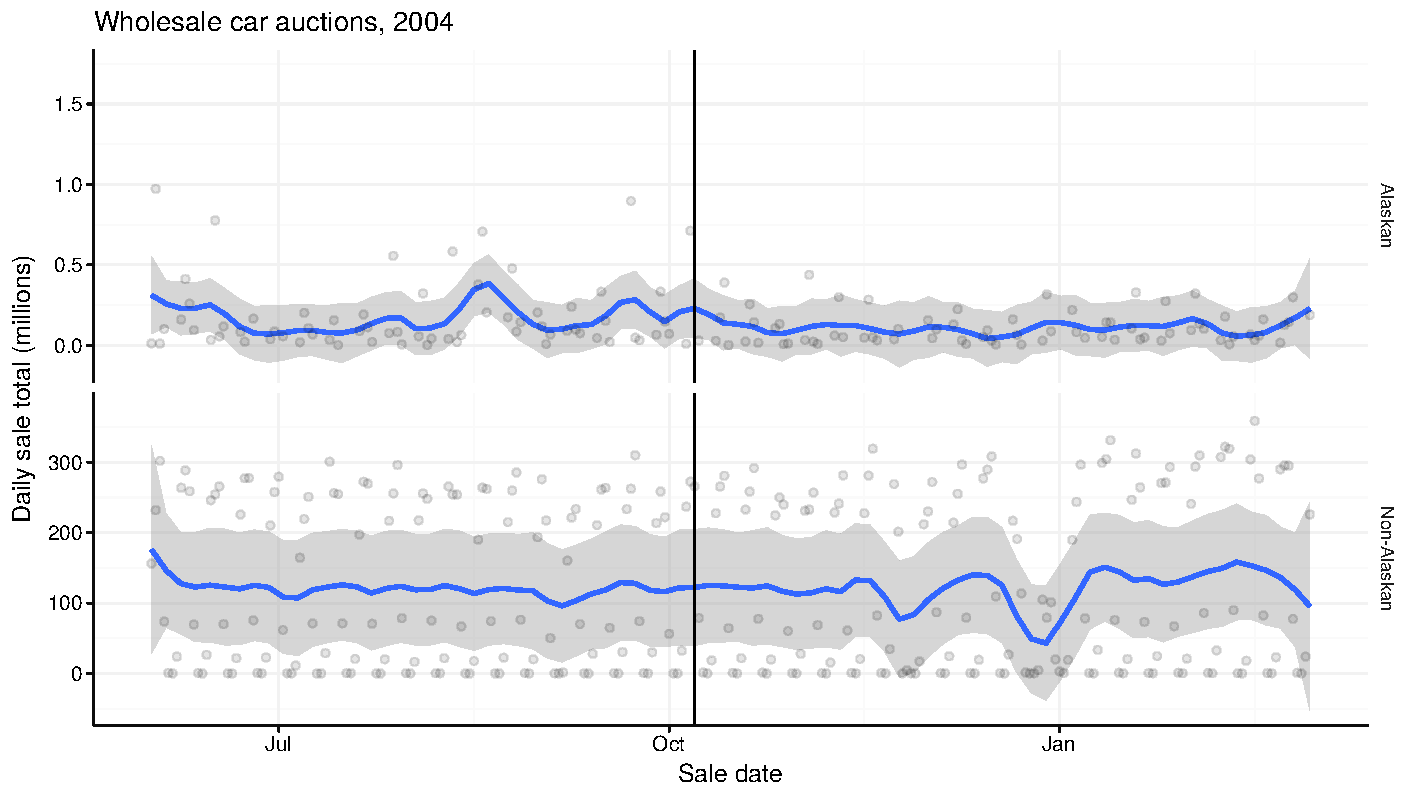
\includegraphics[width=\paperwidth,height=\paperheight]{../Plots/auctions_2004_alaska_vs_other.pdf}}
\begin{frame}[plain]
\end{frame}
}

\begin{frame}{Synthetic Controls!}
\end{frame}


\begin{frame}{Generalized Synthetic Controls!!}
	Synthetic controls, with time-varying factors.

	Depends on $N\to\infty$ and $T\to\infty$.
\end{frame}

\begin{frame}{Xu (2016): election-day registration example}
	\vspace*{-0.1cm}
	\begin{center}
		\includegraphics[page=25, trim = 2.5cm 15.5cm 2.0cm 3.0cm, clip,height=7cm]{../../Papers/Econometrics/Xu_2016.pdf}
	\end{center}
\end{frame}



\end{document}
